\documentclass[conference]{IEEEtran}
\IEEEoverridecommandlockouts
% The preceding line is only needed to identify funding in the first footnote. If that is unneeded, please comment it out.
\usepackage{cite}
\usepackage{amsmath,amssymb,amsfonts}
\DeclareUnicodeCharacter{2009}{\,} 
\usepackage{algorithmic}
\usepackage{graphicx}
\usepackage{hyperref}
\usepackage{textcomp}
\usepackage{xcolor}
\def\BibTeX{{\rm B\kern-.05em{\sc i\kern-.025em b}\kern-.08em
    T\kern-.1667em\lower.7ex\hbox{E}\kern-.125emX}}

\makeatletter
\newcommand{\linebreakand}{%
  \end{@IEEEauthorhalign}
  \hfill\mbox{}\par
  \mbox{}\hfill\begin{@IEEEauthorhalign}
}
\makeatother

\begin{document}

\title{Stellar Classification \textit{vis-à-vis} Convolutional Neural Network\\}

\author{\IEEEauthorblockN{1\textsuperscript{st} Anurag Dutta}
\IEEEauthorblockA{\textit{Department of Computer Science} \\
\textit{Government College of Engineering \& Textile Technology}\\
Serampore, Calcutta, India \\
anuragdutta.research@gmail.com}
\and 
\IEEEauthorblockN{2\textsuperscript{th} Albert Stephan Antony Raj}
\IEEEauthorblockA{\textit{Department of Mathematics}\\
\textit{The Tipsglobal Institute, Bharathiar University, Coimbatore}\\
Coimbatore, Tamil Nadu, India\\
stephanraj138@gmail.com}
\linebreakand
\IEEEauthorblockN{3\textsuperscript{rd} A. Ramamoorthy}
\IEEEauthorblockA{\textit{Department of Mathematics} \\
\textit{Velammal Engineering College, Anna University}\\
Chennai, Tamil Nadu, India \\
ramzenithmaths@gmail.com}
\and
\IEEEauthorblockN{4\textsuperscript{th} John Harshith}
\IEEEauthorblockA{\textit{Department of Computer Science} \\
\textit{Vellore Institute of Technology, Vellore Campus}\\
Vellore, Tamil Nadu, India \\
johnharshith@icloud.com}
\linebreakand
\IEEEauthorblockN{5\textsuperscript{th} Yash Soni}
\IEEEauthorblockA{\textit{Department of Information Technology}\\
\textit{Shri Govindram Seksaria Institute of Technology \& Science}\\
Indore, India\\
yash.work1905@gmail.com}
}

\maketitle

\begin{abstract}
As a result of recent advancements in technology, a variety of new computational fields have emerged. Some examples of these fields are machine learning and intelligence, information science, the internet of things, and others. The advancement of humanity will be greatly aided by these fields. The development of Artificial Intelligence led to the creation of a great deal of Neural Networks. Convolutional Neural Networks are one variation of Neural Networks that we are utilizing in this work. These networks are known to perform quite admirably for Image Categorization, which is one of the purposes for which we are utilizing them. The work encompasses Stellar Classification. There are many stellar entities occupying the region known as universal space. Astrophysicists are familiar with a good number of them, but there are still a great many of these types of entities that have not been discovered yet. Because of the great distance that separates our planet from other stellar entities, any attempt to communicate with them through any channel is highly unlikely to be successful. The most information we could possibly acquire is just a guess as to what kind of entity they are. So, if any scientific observatory comes with a nascent search of any distant entity, we could potentially predict which stellar group they belong to. For the purposes of this work, we are only going to focus on two different types of Stella: Stars and Galaxies. For the purpose of training the Convolutional Neural Network, we have made use of a dataset on Stellar Types with Image Categorization that was created by the Aryabhata Research Institute of Observational Sciences (ARIES), which is located in Nainital, India. This dataset was made publicly available. \\
\end{abstract}

\begin{IEEEkeywords}
Stellar Entities, Galaxy, Stars, Neural Networks, Artificial Intelligence
\end{IEEEkeywords}
\section{Introduction}
The area between celestial bodies [1] and beyond the Earth's surface and its atmosphere is known as outer space [2], also referred to simply as space. In addition to \textit{Electromagnetic Waves}, [3] \textit{Magnetic Forces}, [4] \textit{Neutrinos}, [5] dust, and \textit{Cosmic Rays} [6]. In addition, there is a relatively low concentration of particles in space, the majority of which are a whirlwind of hydrogen and helium, together with other substances such as electromagnetic radiation. The radiation level from \textit{Big Bang} [7] established a temperature of 2.7 kelvins as the standard for the universe. It is believed that approximately half the baryon [8] on this universe is composed of the plasma that exists between galaxies. This plasma has a dynamical temperature that is getting close to millions of kelvin and a number density of fewer than one atom of hydrogen per cubic metre. The accumulation of matter in specific regions leads to the formation of astronomical objects like galaxies and stars. Even though intergalactic space accounts for the vast bulk of the volume of the universe, galaxies and star systems are nevertheless composed of a significant amount of empty space. Dark matter and dark energy are both terms that have been given to refer to an undiscovered form that is thought to account for the vast bulk of the remaining mass-energy found in the physical cosmos. There is no one certain height above the surface of the Earth that marks the beginning of space. In space agreements and for the purpose of keeping aeronautical records, the \textit{Kármán line}, [9] which is an altitude of 100 kilometres above sea level, is traditionally recognised as the starting point of outer space. The term "near space" can also be used to refer to specific regions of the upper stratosphere and the mesosphere. \textit{The Outer Space Treaty}, [10] which went into effect on October 10, 1967, is largely credited with being the document that laid the groundwork for international space law. This convention forbids any government from asserting its right to national sovereignty over outer space and gives all nations the right to freely explore that region. \textit{Anti-satellite weaponry} have been deployed in Earth orbit despite the fact that the United Nations has passed resolutions advocating for the harmonious use of outer space. \\

Space is the only known environment that comes close to being a perfect vacuum [11]. After the initial stage of formation, it essentially has no friction, allowing celestial bodies such as planets, moons, and stars to slide about their ideal orbits with relative ease. The fact that there are only a few atoms of H$_2$ per cubic metre despite the extreme vacuum that exists in intergalactic space is evidence that the region is not entirely empty of material. In comparison, the air that human beings breathe contains approximately 1025 molecules per cubic metre. It may be demonstrated how far electric and magnetic radiations may toil around in space without being scattered by the fact that the mean free path ($\lambda_{mean}$) of any photonic particle in the intergalactic space is approximately $10^{23}$ kilometres, which is equal to 10 billion light years. This is because there is a relatively low concentration of matter in space. Nevertheless, extinction, which is defined as the process of photons being absorbed and scattered by dust and, or gas, continues to be a presidential part of galactic as well as the intergalactic astronomy [12]. \\

Since this work is regarding Stellar Classification, here would be considering only the Stars and the Galaxies in the Outer Space Matrix. A star is a sort of heavenly sphere that is composed of a luminous globe of plasma which is bound in place by the star's intrinsic gravitation. Stars can be distinguished from other types of celestial bodies in a number of ways. The Sun is indeed the astronomical body that orbits the galaxy in the direction opposite that of Earth. At night, there exists a significant number of extra luminaries that are visible with the naked eye. However, because of their enormous distances beyond Earth, these seem as motionless points of light in our night sky. A great number of the sky's brightest stars have been given their own proper names, and the most prominent stars have been arranged into \textit{constellations} [13] and \textit{asterisms} [14]. Astronomers have worked tirelessly to build star catalogues, which list every single known stars and provide conventional designations for stellar names. These catalogues can be found online. It is estimated that there are $10^{22}$ to $10^{24}$ stars in the portion of the universe that can be observed. To the human eye, there are only about 4,000 of these stars visible, and they are all located within the Milky Way galaxy. The gravitational collapse of a gaseous nebula [15] made largely of hydrogen, helium, and traces of heavier elements results in the birth of a star. The primary factor influencing its evolution and ultimate fate is its entire mass. The thermonuclear fusion of hydrogen into helium in a star's core is what keeps it glowing for the majority of its active life. As a result of this process, energy is released into space and travels throughout the star's interior. A star's core eventually decomposes into a stellar remnant, like \textit{White Dwarf} [16], \textit{Black Hole} [17], or \textit{Neutron Star} [18] if the star is sufficiently massive. Almost all chemical elements heavier than lithium that are naturally present are produced by \textit{Stellar Nucleosynthesis} [19] in stars or their remnants. As a result of the explosions of supernovae or the gradual loss of mass by stars, material that has been chemically modified is released back into the interstellar medium. These recycled components are used to construct brand-new stellar bodies. Astronomers are able to determine stellar characteristics such as mass, age, metallicity, variance, distance, and kinematics across space by performing inferences of a star's apparent brightness, spectral response, and modifications in its position in the sky over the course of time. These observations are made possible by the observation of a star's apparent brightness. In the same way that planetary systems and star systems consisting of two or more stars can form orbital systems with one another, so can star systems consisting of other celestial objects. When two such stars are in orbits that are even moderately close to one another, the gravitational interaction between them can have a significant impact on the evolution of both of them. The galaxy and the stellar cluster are both examples of much larger gravitationally coupled systems than individual stars. Galaxies and star clusters both contain stars. \\

A galaxy is made up of a collection of objects that are held together by gravitational forces. These objects include stars, stellar remnants, intergalactic plasma, dust, and antimatter. The name originates from the Greek term galaxias, which simply translates "milky" and alludes to the galaxy known as the Milky Way, in which our solar system is located. Galaxies range in size from dwarfs with fewer than 100 million stars to the largest known galaxies, \textit{SuperGiants} [20] with one hundred trillion stars around their galaxy's centre of mass. Galaxies are thought to have an average of 100 million stars. The stars and nebulae that make up a regular galaxy make up only a small portion of the galaxy's total mass; the vast bulk of the galaxy's mass is made up of something called "dark matter." \textit{SuperMassive} black holes [21] are a typical component of galaxy centres. According to their optical shape, galaxies can be classified as elliptical, spiral, or irregular. It's believed that the centres of several of them contain \textit{SuperMassive} black holes. \textit{Sagittarius A$^*$}, the name of the Milky Way's primary black hole, is four million times more massive than the Sun. \textit{GN-z11} is the oldest and furthest away galaxy as of March 2016. It can be seen as having existed only 400 million years after the Big Bang and is located 32 billion light-years away from Earth. The space in between galaxies is filled with something called the intergalactic medium, which is a very diffuse gas with a density of less than one atom per cubic metre on average. The vast majority of galaxies self-organize into groups, clusters, and \textit{SuperClusters} based on their gravitational interactions. The \textit{Andromeda} Galaxy [22] and the \textit{Milky Way} both play a dominant role in the Local Group, of which the Milky Way is a member. A participant in the \textit{Virgo SuperCluster}, often known as the group. At the largest size, these interactions are often organised into sheets and filaments, which are surrounded by huge voids. \\

In this work, we would make use of Convolutional Neural Network for modelling. The imagery data that is needed to train the model is obtained from \textit{Aryabhata Research Institute of Observational Sciences (ARIES)}. The use of CNN for predicting the class of unidentified stellar entity promises and produces a better accuracy that the traditional classifiers, like Logistic Regression, Random Forest, Decision Tree, k - Nearest Neighbours, Support Vector Machine, etc. In the Results and Conclusion Section of this article, we have provided a comparative analysis of these Classifiers. 
\section{Convolutional Neural Network}
A Convolutional Neural Network [23], often known as a ConvNet, is a type of artificial neural network (ANN) that is typically utilised for the purpose of doing analysis on visual data. Convolutional neural networks are shift-invariant or space-invariant artificial neural networks because their convolution kernels or filters slide along input features and construct translation-equivariant feature maps. Due to the downsampling process that most convolutional neural networks perform on the input, these networks are not invariant to translation. This is contrary to what one may expect. They can improve imagery and video recognition, categorization, dissection, decision support systems, medical imaging analysis, mind interfacing, processing of natural language and financial analysis. \\

Normalized variants of multilayer perceptrons are known as Convolutional Neural Network (CNNs). Typically, when people talk about multilayer perceptrons, they are referring to completely linked networks; this means that every neuron inside one layer has a link to all of the neurons in the following layer. These networks have "full connection," which makes it more likely that they would overfit the data. Regularization, also known as the prevention of overfitting, often involves either reducing connectivity or penalising parameters during training.  Convolutional Neural Networks employ a distinct approach to regularisation in that they make use of the hierarch pattern in the data and construct patterns of increasing the complexity by using smaller and more straightforward patterns imprinted in their filters. In other words, Convolutional Neural Networks take advantage of the hierarchy pattern in the data. As a result, on a scale that measures connectedness and intricacy, Convolutional Neural Networks are located toward the bottom of the scale. The connectivity arrangement between neurons in a convolutional network is designed to imitate the organisation of the visual brain of an animal. This design was motivated by biological processes. The term "receptive field" refers to a certain part of the visual field that is the only one in which individual neurons in the cortex are able to respond to inputs. Because the receptive fields of the many neurons partially overlap one another, the complete visual field can be sensed by the brain. In comparison to certain other image classification methods, CNNs require a minimal amount of pre-processing in order to function. This indicates that the connectivity learns to optimise the filters (or kernels) via autonomous learning, whereas in conventional methods these filtration are hand-engineered. This is in contrast to the fact that the connectivity learns to optimise the filters. One of the most significant benefits is that feature extraction can be done without requiring prior knowledge or the involvement of humans. \\

CNNs have three layers, an \textit{Input Layer}, a \textit{Hidden Layers}, and finally an \textit{Output Layer}. The activation function and final convolution hide the inputs and outputs of feed-forward neural networks' intermediary layers. Convolutional Neural Networks (CNNs) have hidden layers that contain layers that conduct convolutions. In most cases, this will consist of a layer that carries out a dot product of the convolution kernel with the input matrix for the layer. In just about all cases, the \textit{Frobenius} inner product is this product, and the activation function of this product is typically \textit{ReLU}. A feature map is created during the convolution process, and as the convolution kernel moves along the input matrix for the layer, it adds to the input of the following layer. Following this are successive levels, which could include standardizing, pooling, of entirely interconnected tiers, amongst many others.
\section{Dataset}
Located in Nainital, Kumaon, India, the Aryabhatta Research Institute of Observational Sciences (ARIES) is a research organization that focuses on astronomy, solar physics, astrophysics, and atmospheric science. It is a self-governing organisation that operates underneath the Department of Science and Technology of the Indian government. ARIES is conducting research on a variety of areas associated with the sun, stars, and galaxies. ARIES has made a number of important contributions to the scientific community, most notably in the fields of star clusters and gamma-ray bursts (GRBs). In this article, the Convolutional Neural Network is proposed to be trained by using an imagery dataset of Stellar Objects. ARIES helped us with such an observatory dataset. The dataset is made freely available at \href{https://github.com/Anurag-Dutta/Stellar-Classification-vis---vis-Convolutional-Neural-Network/tree/main/dataset}{https://github.com/Anurag-Dutta/Stellar-Classification-vis---vis-Convolutional-Neural-Network/tree/main/dataset}. The dataset is divided mainly into two categories - Stars and Galaxies. Figure 1 shows a pictorial glimpse of a few imagery data points for the category - Galaxy. 
\begin{figure}[htbp]
\label{fig1}
\centerline{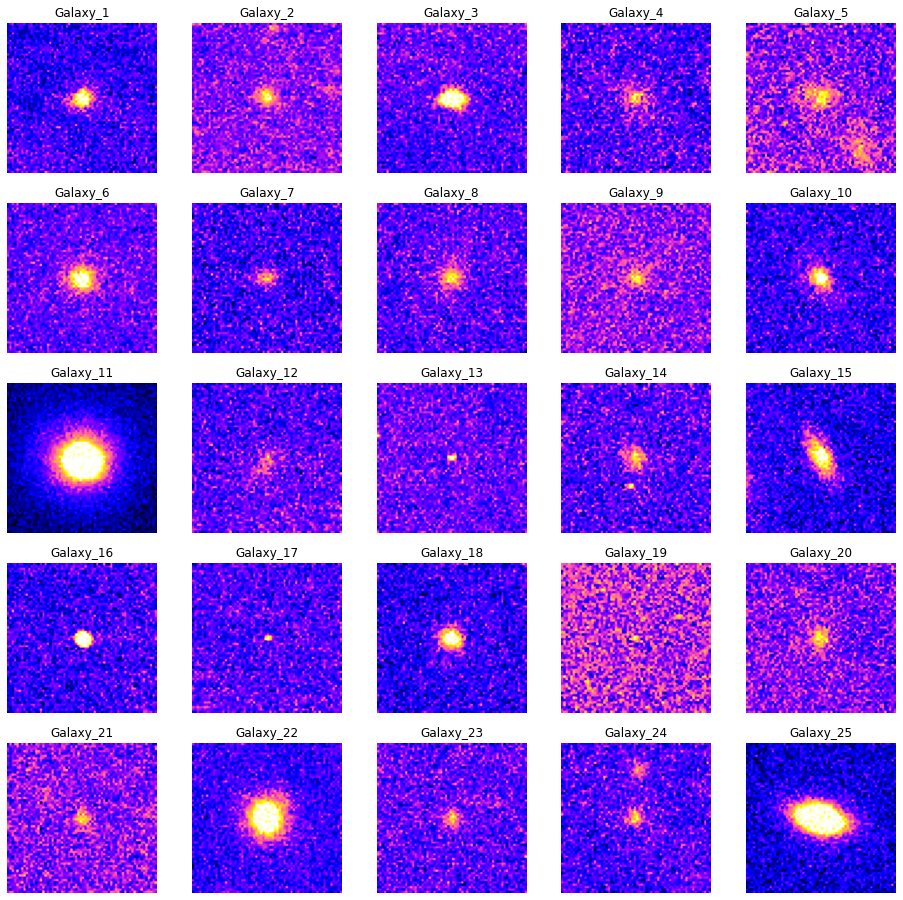
\includegraphics[width = \linewidth]{1}}
\caption{A Glimpse of 25 amongst 942 data points under \textit{Galaxial} Category from the ARIES Imagery Dataset. }
\end{figure}
Figure 2 shows a pictorial glimpse of a few imagery data points for the category - Galaxy. 
\begin{figure}[htbp]
\label{fig2}
\centerline{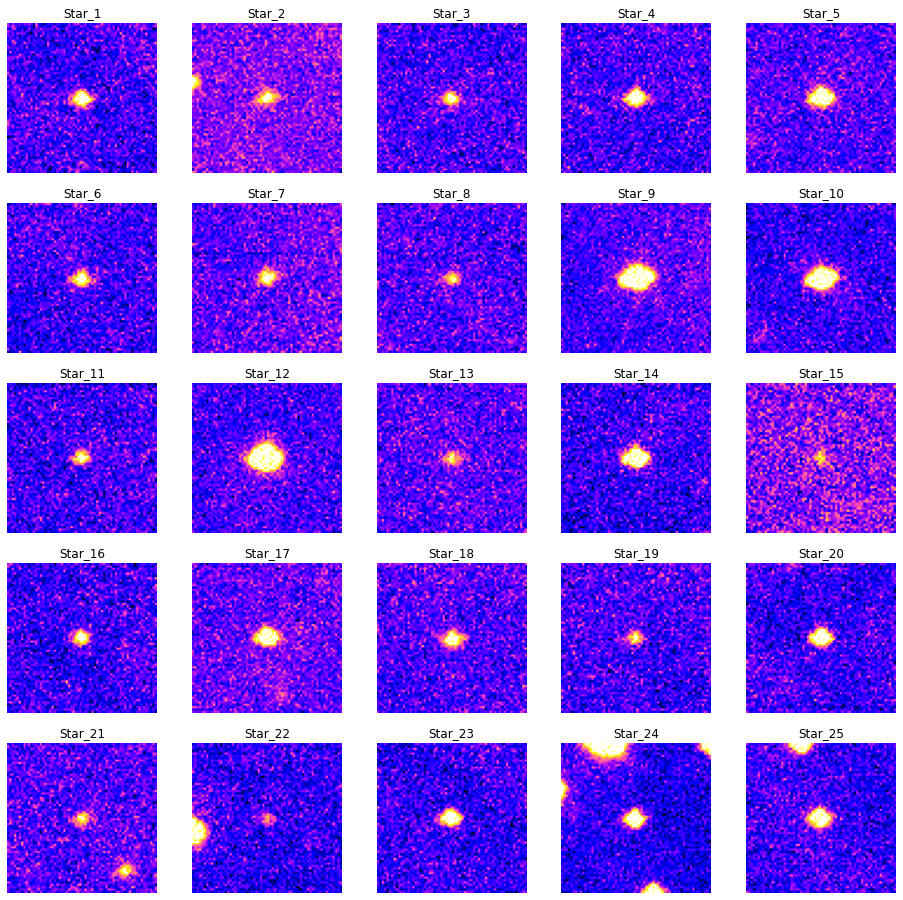
\includegraphics[width = \linewidth]{2}}
\caption{A Glimpse of 25 amongst 3044 data points under \textit{Stellar} Category from the ARIES Imagery Dataset. }
\end{figure}
\section{Results and Conclusion}
In this section, we would conclude the works and discussions thrown about in this article. We would also compare the Classification performance of different Models. Firstly, we made use of Traditional Classifiers, like Naive Bayes, SVm, etc. The results were as, 
\begin{verbatim}
==========================
[ Support Vector Machine ]
==========================

--------
TRAINING
--------

Training F1 Score = 0.9416562107904642

-------
TESTING
-------

Testing F1 Score = 0.7982456140350878
Precision = 0.7984189723320159
Recall = 0.9869706840390879
F1 Score = 0.8827385287691187

\end{verbatim}
\begin{verbatim}
==========================
[ Random Decision Forest ]
==========================

--------
TRAINING
--------

Training F1 Score = 1.0

-------
TESTING
-------

Testing F1 Score = 0.8145363408521303
Precision = 0.8123324396782842
Recall = 0.9869706840390879
F1 Score = 0.8911764705882353

\end{verbatim}
\begin{verbatim}
=================
[ Decision Tree ]
=================

--------
TRAINING
--------

Training F1 Score = 1.0

-------
TESTING
-------

Testing F1 Score = 0.7518796992481203
Precision = 0.8354838709677419
Recall = 0.8436482084690554
F1 Score = 0.8542635658914729

\end{verbatim}
\begin{verbatim}
========================
[ Gaussian Naive Bayes ]
========================

--------
TRAINING
--------

Training F1 Score = 0.7020075282308658

-------
TESTING
-------

Testing F1 Score = 0.6766917293233082
Precision = 0.7956810631229236
Recall = 0.7801302931596091
F1 Score = 0.7878289473684211

\end{verbatim}
\begin{verbatim}
==========================
[ k - Nearest Neighbours ]
==========================

--------
TRAINING
--------

Training F1 Score = 0.8252823086574655

-------
TESTING
-------

Testing F1 Score = 0.7957393483709273
Precision = 0.8043184885290149
Recall = 0.9706840390879479
F1 Score = 0.8797047970479704

\end{verbatim}
Amongst all the traditional Classifiers, the Random Forest Classifier performed the best. Figure 3 and 4 shows the Precision Recall Curve and the Confusion Matrix for the Random Forest Model.
\begin{figure}[htbp]
\label{fig3}
\centerline{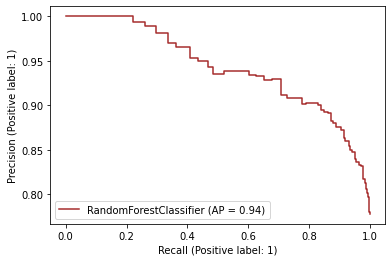
\includegraphics[width = \linewidth]{3}}
\caption{Precision Recall Variation for the Random Forest Classifier}
\end{figure}
\begin{figure}[htbp]
\label{fig4}
\centerline{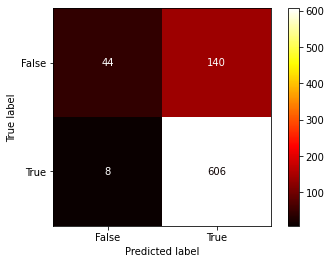
\includegraphics[width = \linewidth]{4}}
\caption{Confusion Matrix for the Random Forest Classifier}
\end{figure}

But, we could definitely be better by making use of the Convolutional Neural Network. We made use of $\mathtt{Sequential}$ model, and $\mathtt{ReLU}$ as an activation function for modelling the CNN. The training to the CNN is done in normalized batches. For that, we utilized the $\mathtt{BatchNormalization()}$ functionality. We also padded the training samples. Padding is introduced to the image's frame so that the kernel has extra room to work on the image while it is being processed. This is done to provide the kernel with a helping hand in the processing of the image. The ability to perform more precise image analysis is enabled by feeding padding into a CNN that is processing an image. For that, we introduced $\mathtt{padding='valid'}$ as a parameter for modelling the CNN. For traversal, we selected a stride of 2. As the training was done in batches, we fitted the data as $\mathtt{epochs}$. For fitting the CNN, here in this work, we considered $\mathtt{epochs=10}$. Figure 5 and 6 shows the contrast in accuracy and loss respectively, for the CNN Model while Training and Testing for different $\mathtt{epochs}$.
\begin{figure}[htbp]
\label{fig5}
\centerline{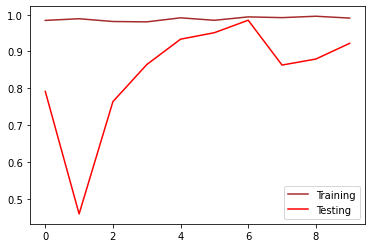
\includegraphics[width = \linewidth]{5}}
\caption{Variation of accuracy for the CNN Model for different $\mathtt{epochs}$}
\end{figure}
\begin{figure}[htbp]
\label{fig6}
\centerline{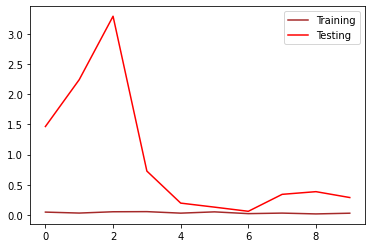
\includegraphics[width = \linewidth]{6}}
\caption{Variation of loss for the CNN Model for different $\mathtt{epochs}$}
\end{figure}
The highest validation accuracy was attained by the CNN Model at 10$^{th}$ $\mathtt{epoch}$ that was 0.9221. A summary of the last $\mathtt{epochs}$ foe fitting the model is 
\begin{verbatim}
Epoch 10/10
loss: 0.0257
accuracy: 0.9907
val_loss: 0.2861
val_accuracy: 0.9221
\end{verbatim}
On a whole, the Convolutional Neural Network works well for this scenario with an accuracy of nearly 92\%. Though, increasing the number of $\mathtt{epochs}$ will ensure higher accuracy, but the computational time will increase.
\begin{thebibliography}{00}
\bibitem{b1} F. Yoshida and T. Nakamura, “Size Distribution of Faint Jovian L4 Trojan Asteroids,” \textit{The Astronomical Journal}, vol. 130, no. 6, pp. 2900–2911, Dec. 2005, doi: 10.1086/497571.
\bibitem{b2} G. LEMAÎTRE, “The Beginning of the World from the Point of View of Quantum Theory,” \textit{Nature}, vol. 127, no. 3210, pp. 706–706, May 1931, doi: 10.1038/127706b0.
\bibitem{b3} S. Chen, A. Maksimchuk, and D. Umstadter, “Experimental observation of relativistic nonlinear Thomson scattering,” \textit{Nature}, vol. 396, no. 6712, pp. 653–655, Dec. 1998, doi: 10.1038/25303.
\bibitem{b4} K. Tuchin, “Particle Production in Strong Electromagnetic Fields in Relativistic Heavy-Ion Collisions,” \textit{Advances in High Energy Physics}, vol. 2013, pp. 1–34, 2013, doi: 10.1155/2013/490495.
\bibitem{b5} “Search for Majorana neutrinos with the first two years of EXO-200 data,” \textit{Nature}, vol. 510, no. 7504, pp. 229–234, Jun. 2014, doi: 10.1038/nature13432.
\bibitem{b6} S. VERNOFF, “Radio-Transmission of Cosmic Ray Data from the Stratosphere,” \textit{Nature}, vol. 135, no. 3426, pp. 1072–1073, Jun. 1935, doi: 10.1038/1351072c0.
\bibitem{b7} J. P. Huchra, “The Hubble Constant,” \textit{Science}, vol. 256, no. 5055, pp. 321–325, Apr. 1992, doi: 10.1126/science.256.5055.321.
\bibitem{b8} J. P. Macquart et al., “A census of baryons in the Universe from localized fast radio bursts,” \textit{Nature}, vol. 581, no. 7809, pp. 391–395, May 2020, doi: 10.1038/s41586-020-2300-2.
\bibitem{b9} P. Voosen, “Outer space may have just gotten a bit closer,” \textit{Science}, Jul. 2018, doi: 10.1126/science.aau8822.
\bibitem{b10} M. Bourbonniere and R. J. Lee, “Legality of the Deployment of Conventional Weapons in Earth Orbit: Balancing Space Law and the Law of Armed Conflict,” \textit{European Journal of International Law}, vol. 18, no. 5, pp. 873–901, Nov. 2007, doi: 10.1093/ejil/chm051.
\bibitem{b11} E. J. Öpik, “The lunar atmosphere,” \textit{Planetary and Space Science}, vol. 9, no. 5, pp. 211–244, May 1962, doi: 10.1016/0032-0633(62)90149-6.
\bibitem{b12} T. E. Collett et al., “A precise extragalactic test of General Relativity,” \textit{Science}, vol. 360, no. 6395, pp. 1342–1346, Jun. 2018, doi: 10.1126/science.aao2469.
\bibitem{b13} J. P. Britton, “Studies in Babylonian lunar theory: part III. The introduction of the uniform zodiac,” \textit{Archive for History of Exact Science}s, vol. 64, no. 6, pp. 617–663, Sep. 2010, doi: 10.1007/s00407-010-0064-z.
\bibitem{b14} M. Odenkirchen and C. Soubiran, “NGC 6994 – clearly not a physical stellar ensemble,” \textit{Astronomy \& Astrophysics}, vol. 383, no. 1, pp. 163–170, Feb. 2002, doi: 10.1051/0004-6361:20011730.
\bibitem{b15} C. J. Davis, M. D. Smith, T. M. Gledhill, and W. P. Varricatt, “Near-infrared echelle spectroscopy of protoplanetary nebulae: probing the fast wind in H2,” \textit{Monthly Notices of the Royal Astronomical Society}, vol. 360, no. 1, pp. 104–118, Jun. 2005, doi: 10.1111/j.1365-2966.2005.09018.x.
\bibitem{b16} R. de la Fuente Marcos and C. de la Fuente Marcos, “Deep and fast Solar System flybys: the controversial case of WD 0810-353,” \textit{Astronomy \& Astrophysics}, vol. 668, p. A14, Nov. 2022, doi: 10.1051/0004-6361/202245020.
\bibitem{b17} M. Caleb et al., “Discovery of a radio - emitting neutron star with an ultra-long spin period of 76 s,” \textit{Nature Astronomy}, vol. 6, no. 7, pp. 828–836, May 2022, doi: 10.1038/s41550-022-01688-x.
\bibitem{b18} R. Campos Delgado, “Quantum gravitational corrections to the entropy of a Reissner–Nordström black hole,” \textit{The European Physical Journal C}, vol. 82, no. 3, Mar. 2022, doi: 10.1140/epjc/s10052-022-10232-0.
\bibitem{b19} E. G. Adelberger et al., “Solar fusion cross sections II: the pp chain and CNO cycles,” \textit{Reviews of Modern Physics}, vol. 83, no. 1, pp. 195–245, Apr. 2011, doi: 10.1103/RevModPhys.83.195.
\bibitem{b20} J. D. Lyman, D. Bersier, and P. A. James, “Bolometric corrections for optical light curves of core-collapse supernovae,” \textit{Monthly Notices of the Royal Astronomical Societ}y, vol. 437, no. 4, pp. 3848–3862, Dec. 2013, doi: 10.1093/mnras/stt2187.
\bibitem{b21} F. Pacucci and A. Loeb, “Separating Accretion and Mergers in the Cosmic Growth of Black Holes with X-Ray and Gravitational-wave Observations,” \textit{The Astrophysical Journal}, vol. 895, no. 2, p. 95, Jun. 2020, doi: 10.3847/1538-4357/ab886e.
\bibitem{b22} W. Liller and B. Mayer, “The rate of nova production in the Galaxy,” \textit{Publications of the Astronomical Society of the Pacific}, vol. 99, p. 606, Jul. 1987, doi: 10.1086/132021.
\bibitem{b23} O. Avilov, S. Rimbert, A. Popov, and L. Bougrain, “Deep Learning Techniques to Improve Intraoperative Awareness Detection from Electroencephalographic Signals,” \textit{2020 42nd Annual International Conference of the IEEE Engineering in Medicine \& Biology Society (EMBC)}, Jul. 2020, doi: 10.1109/embc44109.2020.9176228.
\end{thebibliography}
\end{document}
